\documentclass[appendixprefix,a4paper,bibliography=totoc,twoside=true,11pt,DIV=11,BCOR=6mm,headsepline,pointlessnumbers]{scrbook}
\usepackage[ngerman]{babel}

\usepackage[T1]{fontenc}
\usepackage[utf8]{inputenc}
%\usepackage{amsmath, amsthm, amssymb} %Formatierung der Formeln von MPues 
\usepackage{amsmath,amssymb,amsthm,upgreek,bbm,textcomp,mhchem,siunitx}
\usepackage{mathtools}
\usepackage{bibgerm}
\usepackage{graphicx} 
%\graphicspath{{./src/}} 		
\usepackage[marginal, hang]{footmisc}        %F�r andere Fu�noten. Doku: 
%http://www.cs.brown.edu/system/software/latex/doc/footmisc.pdf, MUSS VOR setspace geladen werden
\usepackage{setspace}                        %f�r 1,5er Zeilenabstand
%\usepackage{longtable}
%\usepackage[automark]{scrpage2}
%\usepackage{lineno}                        %Zeilennummerierung
\usepackage{esvect}                            %Vektorpfeile: Benutzung mit \vv{abc}
%\usepackage{subfig}                         %Mehrere Bilder
%\SI{6,1}{\giga\hertz}.
\usepackage{lmodern}                        %latin modern schriftarten laden
\usepackage{color}                            %Farbiger Text in Tex. Benutzen mit \textcolor[red}{hier der text}
%\usepackage{booktabs}                        %F�r Excel2Latex
\usepackage{multirow}
%\usepackage{bigfoot}
\usepackage[labelfont=bf, format=plain, font=small]{caption}
\usepackage[rightcaption]{sidecap}
\usepackage[hyperfootnotes=false]{hyperref}                        
%links in pdf erzeugen, als letztes Paket setzten sonst gibts mit pagenumbering stress
\usepackage[babel,german=quotes]{csquotes}        % F�r einheitliche Anf�hrungszeichen
\usepackage{placeins} %F�r Float-Barrier und Kontrolle �ber Floating-Objekte
%\usepackage{algorithm2e}
%\usepackage{algpseudocode}

%\usepackage[firstpage]{draftwatermark}
%\usepackage{draftwatermark}

\usepackage{algpseudocode}
\usepackage[Algorithmus]{algorithm}
% \usepackage[Algorithmus]{algorithm}
% \usepackage{algorithmicx}
% \usepackage{algcompatible}
% \usepackage{algorithm2e}
\usepackage{ragged2e}

%\renewcommand{\sffamily}{\fontfamily{phv}\selectfont}          %�berschriften in Helvetica

\begin{document}
%%%%%%%%%%%%%%%%%%%%%%%%%%%%%%%%%%%%%%%%%%%%%%%%%%%%%%%%%%%%
%Schalter Titelseite
%
% \titlehead{titlehead}%
% \subject{}
% \subtitle{}
%
\title{Implementierung von Skelett-Algorithmen mit dem Kinect-Sensor}
\author{Arbeitsbereich Kognitive Systeme (KOGS)\\ Fachbereich Informatik\\ Universität Hamburg}
\publishers{Projektbarbeit\\ Projekt Bildverarbeitung \\Johannes Böhler, Christopher Kroll, Sandra Schröder\\  \vspace{2 cm} Sommersemester 2012 bis Wintersemester 2012/2013}
%\uppertitleback{uppertitleback}
\lowertitleback{}
\date{}
%%%%%%%%%%%%%%%%%%%%%%%%%%%%%%%%%%%%%%%%%%%%%%%%%%%%%%%%%%%%%
%
% 
% \begin{titlepage}
% \thispagestyle{empty}
% \begin{center}
% 
% {\LARGE Bachelorarbeit: \\ [1cm]
% Ballerkennung mit Formwahrscheinlichkeitsverteilungen im Robocup\\[2cm] }
% 
% {\Large von
% \\ [0.5cm]  Sandra Schröder\\
% (6060939)\\
% geboren am \\ 12.05.1989\\ [2cm]}
% 
% {\Large im Studiengang
% Informatik\\
% Arbeitsbereich Technische Informatiksysteme \\
% Universit\"at Hamburg\\[3cm]}
% 
% 
% \end{center}
% Erstgutachter: Prof. Dr.-Ing. Dietmar P. F. Möller\\
% Zweitgutachter: Prof. Dr. rer. nat. Leonie Dreschler-Fischer
% \end{titlepage}
\maketitle
\chapter{Einleitung}
\chapter{Aufgabenstellung}
\section{Die Kinect-Funktionsweise}
\subsection{Funktionsweise}
Die drei Haupt Hardware-Komponenten der Kinect sind ein Infrarot Projektor, eine Infrarot Kamera sowie eine Infrarot Kamera.

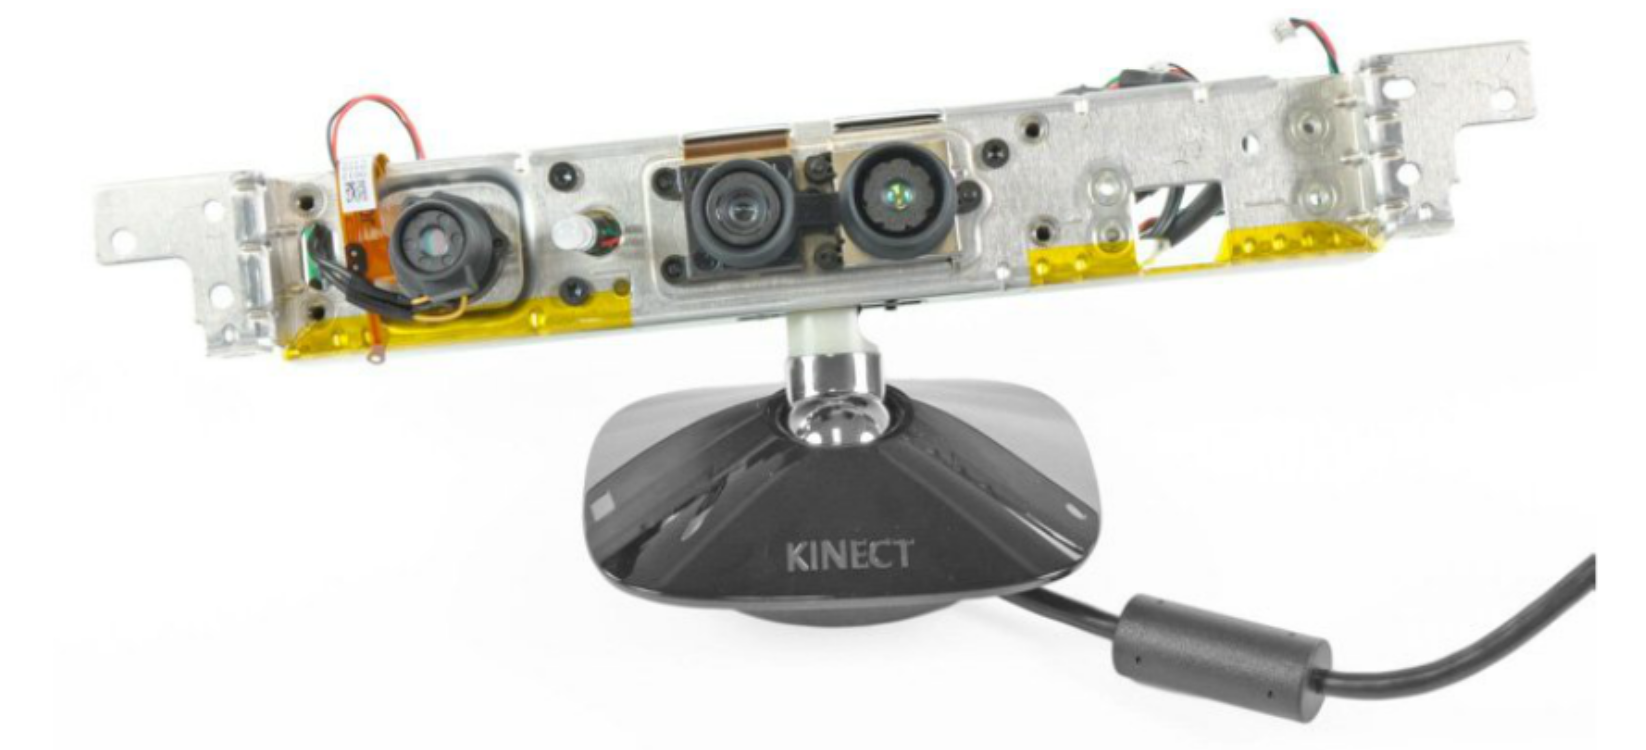
\includegraphics[height=5cm]{Res/Kinect_Components.png}



Die Kombination aus Infrarot Strahler und Infrarot Kamera ermöglicht die Gewinnung von Tiefeninformationen aus der Umgebung. Im Gegensatz zu gewöhnlichen Kameras welche einem Pixel Farbinformation (z.B.  über RGB-Farbkanäle) zuordnen, wird dem Pixel mit Hilfe der Infrarot Kamera eine Entfernung zugeordnet. Diese ergibt sich aus der Art und Weise wie der Infrarotstrahl von dem durch den Pixel repräsentierten Bereich eines Objektes reflektiert wurde.

Die Tiefenbilder welche man von der IR Kamera erhält, sehen aus wie komplett verrauschte Graustufenbilder. Hierbei steht jeder Grau Wert eines Pixels für die entsprechende Entfernung des korrespondierenden Objektausschnittes zur Kinect.



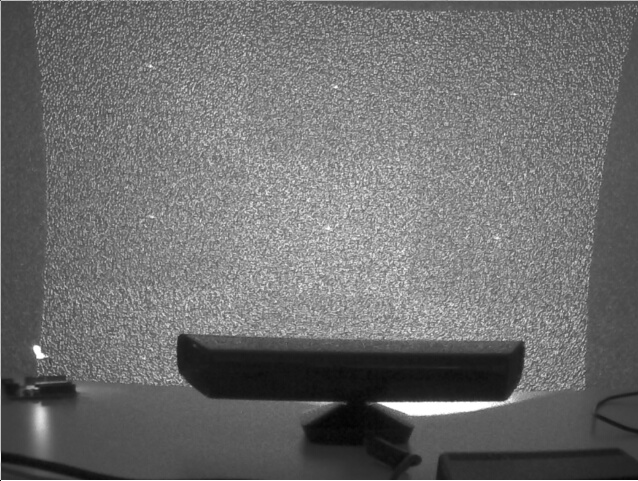
\includegraphics[height=5cm]{Res/Kinect_9Points.png}



Hohe Grauwerte (helle Pixel) repräsentieren nahe Objekte während niedrige Grauwerte (dunkle Pixel) weiter entfernte Objekte beschreiben. In einem Tiefenbild ist die gesamte Information über die Entfernung der im Bildausschnitt erfassten Objekte zur Kinect enthalten.

Wird die Tiefeninformation dazu genutzt um die Pixel mit Hilfe der durch die RGB Kamera erfassten Farbwerte der XY Koordinaten im dreidimensionalen Raum anzuordnen, erhält man eine sogenannte (farbige) Punktwolke. Die in der 2d 
-Betrachtung benachbarte Pixel müssen in der 3d Repräsentation nicht miteinander verbunden da die Z-Koordinate unterschiedliche Werte aufweisen kann.
\subsection{Funktionale Komponenten}
\subsubsection{Infrarotprojektor}

Der Infrarotprojektor emittiert elektromagnetische Strahlen, deren Wellenlänge (830nm) außerhalb des für den Menschen sichtbaren Bereichs liegt (380nm-780nm).
Der Projektor strahlt zur Tiefenbestimmung ein Gitter von Infrarotpunkten (strukturiertes Licht) auf die Objekte in seiner Umgebung ab. 
Die Firma PrimeSense (welche von Microsoft aufgekauft wurde) implementiert ein besonderes Verfahren zur Generierung dieses Musters.
Normalerweise produzieren Filter die diese Art von Muster generieren einen sehr hellen Punkt in der Mitte des Bildes, welcher die Leistungsfähigkeit des IR Projektors limitiert.\\


Durch das hier angewandte Verfahren entstehen statt einem einzigen sehr hellen, neun helle Punkte, welche durch unvollständige Lichtfilterung zur Mustererstellung bedingt sind. Das hier eingesetzte Verfahren produziert weniger starke Artefakte und ermöglicht die Verwendung einer leistungsfähigeren Diode was eine erhöhte Genauigkeit sowie eine größere Reichweite ermöglicht. . Trotzdem ist die Reichweite des IR Projektors eingeschränkt, da zu hohe Intensitäten der IR Strahlen Augenschäden verursachen könnten.


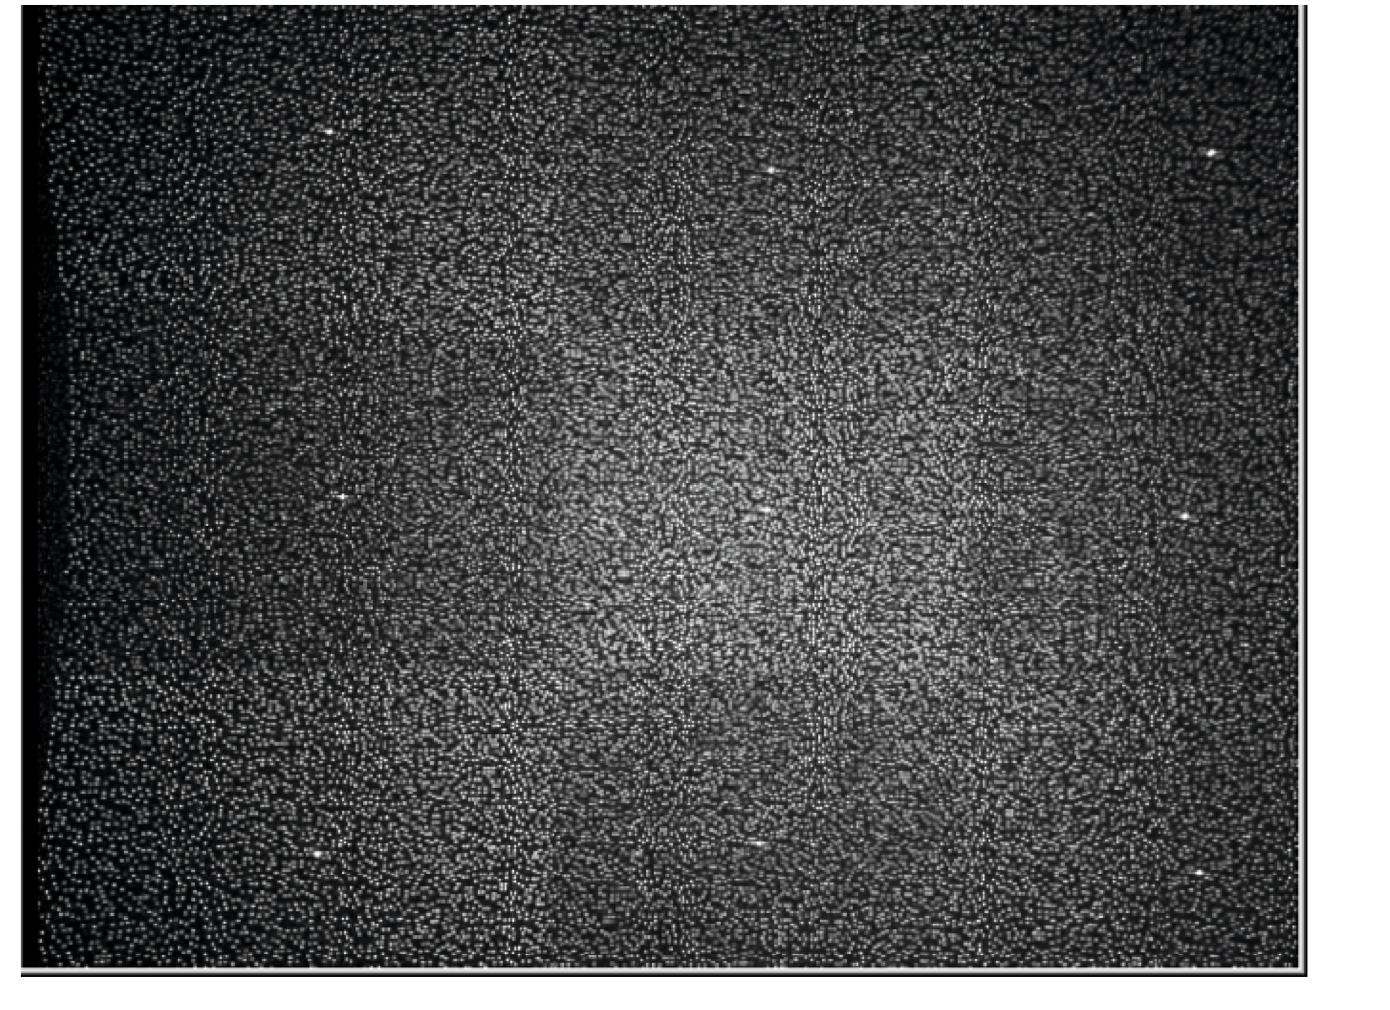
\includegraphics[height=5cm]{Res/9_Dots.png}



Es ist wichtig dass die Wellenlänge der Infrarot strahlen konstant bleibt, was durch eine konstante Temperatur der Laserdiode und eine konstante Stromleistung (60 mW) gewährleistet wird. Problem hierbei sind variierende Außentemperaturen(die empfohlene Betriebstemperatur  liegt zwischen 5 und 35 °C). Um diese Konstanz zu gewährleisten wird ein sogenanntes  Peltier-Element verwendet, welches sowohl kühlen als auch wärmen kann.\\

\subsubsection{Infrarotkamera}


Die IR Kamera nimmt Bilder mit einer nativen Auflösung von 1280x1024 Pixeln bei einer Bildwiederholrate von 30 Hz auf. Weitergeleitet werden allerdings nur Bilder mit einer Auflösung von 640x480 Pixeln da der USB Datenbus eine Limitierung bezüglich übertragbarer Datenraten darstellt. Das Blickfeld der IR Kamera beträgt in der Horizontalen 58 °, in der Vertikalen 45 °. Damit sich die Mustererkennung funktioniert ist eine Mindestabstand von 0,8 Metern erforderlich, ab einer Entfernung von 3,5 Metern wird die Intensität der reflektierten Strahlen zu gering um Tiefeninformationen mit ausreichender Präzision zu erhalten.\\

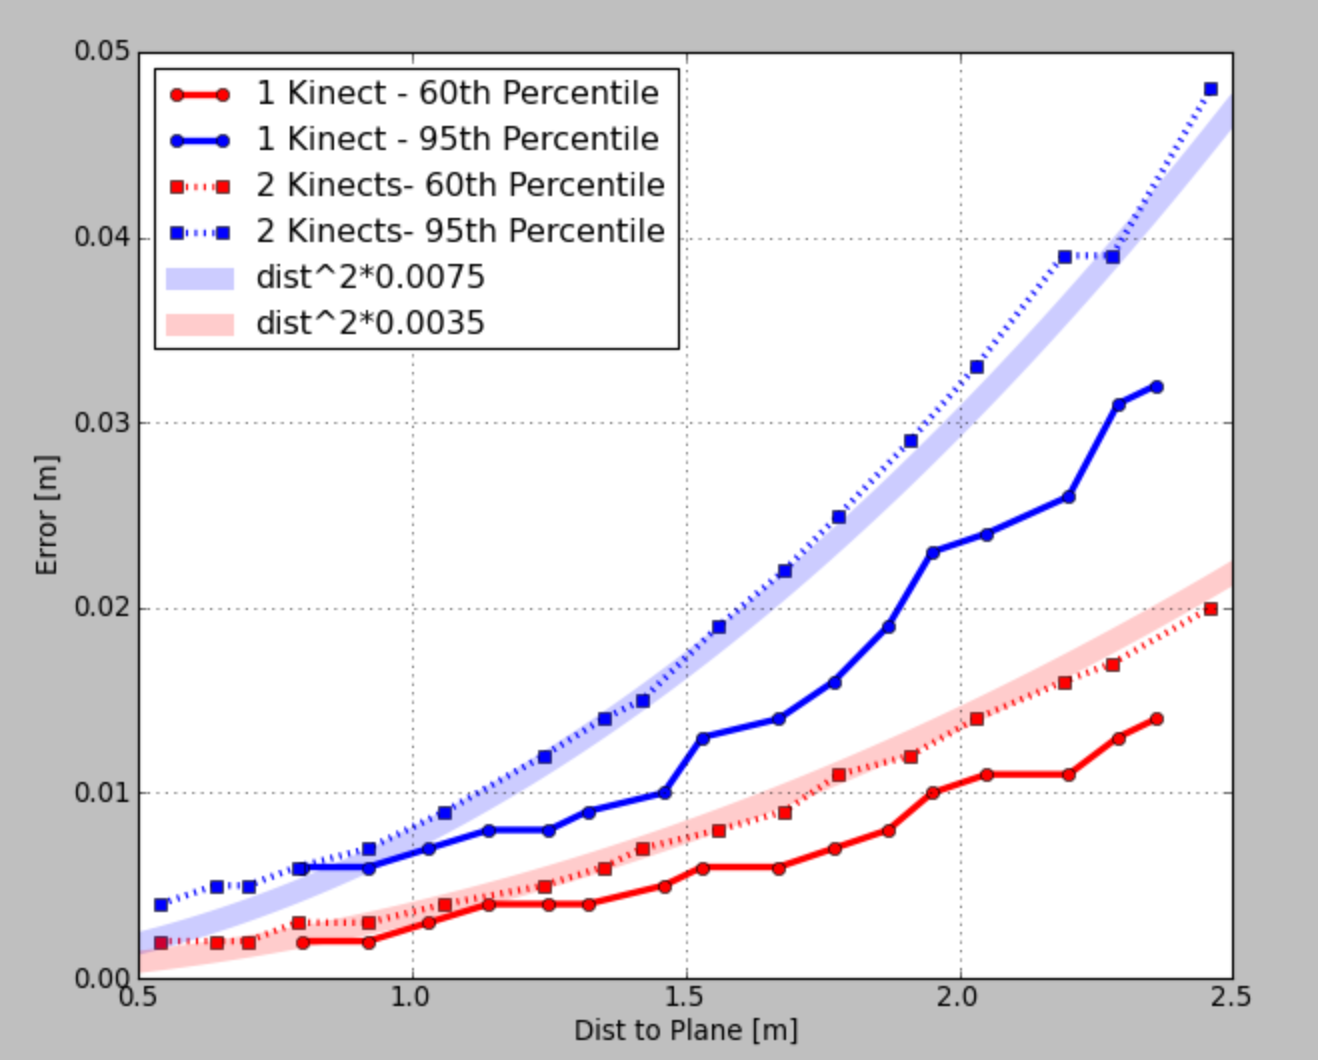
\includegraphics[height=5cm]{Res/Res_to_Dist.png}

Bei einem optimalen Abstand von 2 Metern zum Objekt beträgt die Auflösung in der XY Ebene 3mm, in der Z Ebene 1cm.
Die Quantisierungsauflösung liegt bei  (2048) Bit.
Es muss sichergestellt werden dass die IR Kamera nur die erwünschte elektromagnetische Strahlung im 830 nm Bereich aufnimmt und nicht von Strahlungen anderer Wellenlänge gestört wird . Die wird durch einen Filter welcher auf dem IR Kameraobjektiv angebracht ist realisiert.
Trotz des Filters sollte die Kinect eher in abgedunkelten Innenräumen verwendet werden, da im Sonnenlicht auch elektromagnetische Wellen im Infrarotbereich enthalten sind.\\

\subsubsection{RGB Kamera}

Die RGB Kamera nimmt bei einer Wiederholrate von 30 Hz ebenfalls mit einer Auflösung von 640x480 Pixeln auf, könnte aber alternativ auch mit einer Auflösung von 1280x1024 Pixeln bei einer reduzierten Wiederholrate von 15 Bildern pro Sekunde angesteuert werden.
Die Quantisierungsauflösung liegt hier bei  (256)Bit. \\


\subsubsection{Mikrofon Array}
Die Kinect beinhaltet vier Mikrofone welche verteilt verbaut sind. Sie dienen sowohl der Erfassung von Ton, als auch der Lokalisierung und Unterscheidung von Soundquellen. Jedes der Mikrophone tastet mit einer Quantisierungsauflösung von  (65536) Bit und einer Abtastrate von 16 KHz ab.

\subsection{Tiefenberechnung}

Die Berechnung der Objektentfernungen (Tiefenwerte) innerhalb der Kinect erfolgt durch Aussendung von strukturiertem Licht durch die Projektionseinheit und durch Weiterverwertung  der durch die IR empfangen reflektierten Strahlen auf einem Chip der Firma PrimeSense (PS1080-A2-Chip). Das Muster für das strukturierte Licht wird mit Hilfe eines Diffusors(einer Lochplatte mit fest definiertem Muster) erzeugt.\\
Das Prinzip des Strukturierten Lichts ist an ein Verfahren angelehnt, welches sich Streifenprojektion nennt und in dieser Anwendung abgewandelt wurde um die Erfassung von beweglichen Objekten zu ermöglichen. Statt Lichtstreifen wird bei dem von der Kinect angewendeten Verfahren eine Punktematrix verwendet, welche fest definiert ist. Die IR Kamera sowie der Projektor müssen sich hierzu in einem fest definiertem, gleich großem Abstand zueinander befinden.
Die Umgebungsreflektionen der projizierten Punktematrix werden von der Infrarotkamera erfasst.
Um aus diesem Gitter von Infrarotpunkten Tiefeninformation extrahieren zu können wird das Verfahren der aktiven Stereotriangulation verwendet.\\


Die Triangulation ist ein Verfahren zur optischen Abstandsmessung welches sich hierzu trigonometrischer Funktionen innerhalb von aufgespannten Dreiecken bedient. 
Es wird allgemein zwischen aktiver und passiver Triangulation unterschieden.
Aktive Triangulation bedeutet dass mindestens eine strukturierte Lichtquelle zur Abstandsberechnung erforderlich ist, während dies bei passiver Triangulation nicht der Fall ist.
Da der IR Projektor ein statisches Pseudozufallsmuster emittiert, ist dieser als strukturierte Lichtquelle einzuordnen.
Stereotriangulation bedeutet dass zwei unterschiedliche Bildquellen benötigt werden um die Tiefe jedes Pixels eines Bildausschnittes berechnen zu können.
Eine Bildquelle ist der Diffusor (das „Lochmuster“) welcher die vom Projektor emittierten Strahlen statisch definiert. Die andere Bildquelle ist die IR Kamera.
Das erste Bild ist immer identisch und statisch, das zweite hingegen variiert je nach Umgebung. Diese beiden Bilder sind die Grundlage für die trigonometrischen Operationen zur Berechnung der Tiefeninformationen. Hierzu wird die horizontale Differenz des Punktes Y1 des von der IR Kamera aufgenommenen Bildes zum korrespondierenden Punkt Y2 des virtuellen statischen Referenzbildes des Projektors berechnet. Aus dieser Differenz lässt sich die Tiefe des betreffenden Pixels durch aufstellen der beiden Projektionslinien und Schnittpunktbestimmung derselben berechnen. \\
 


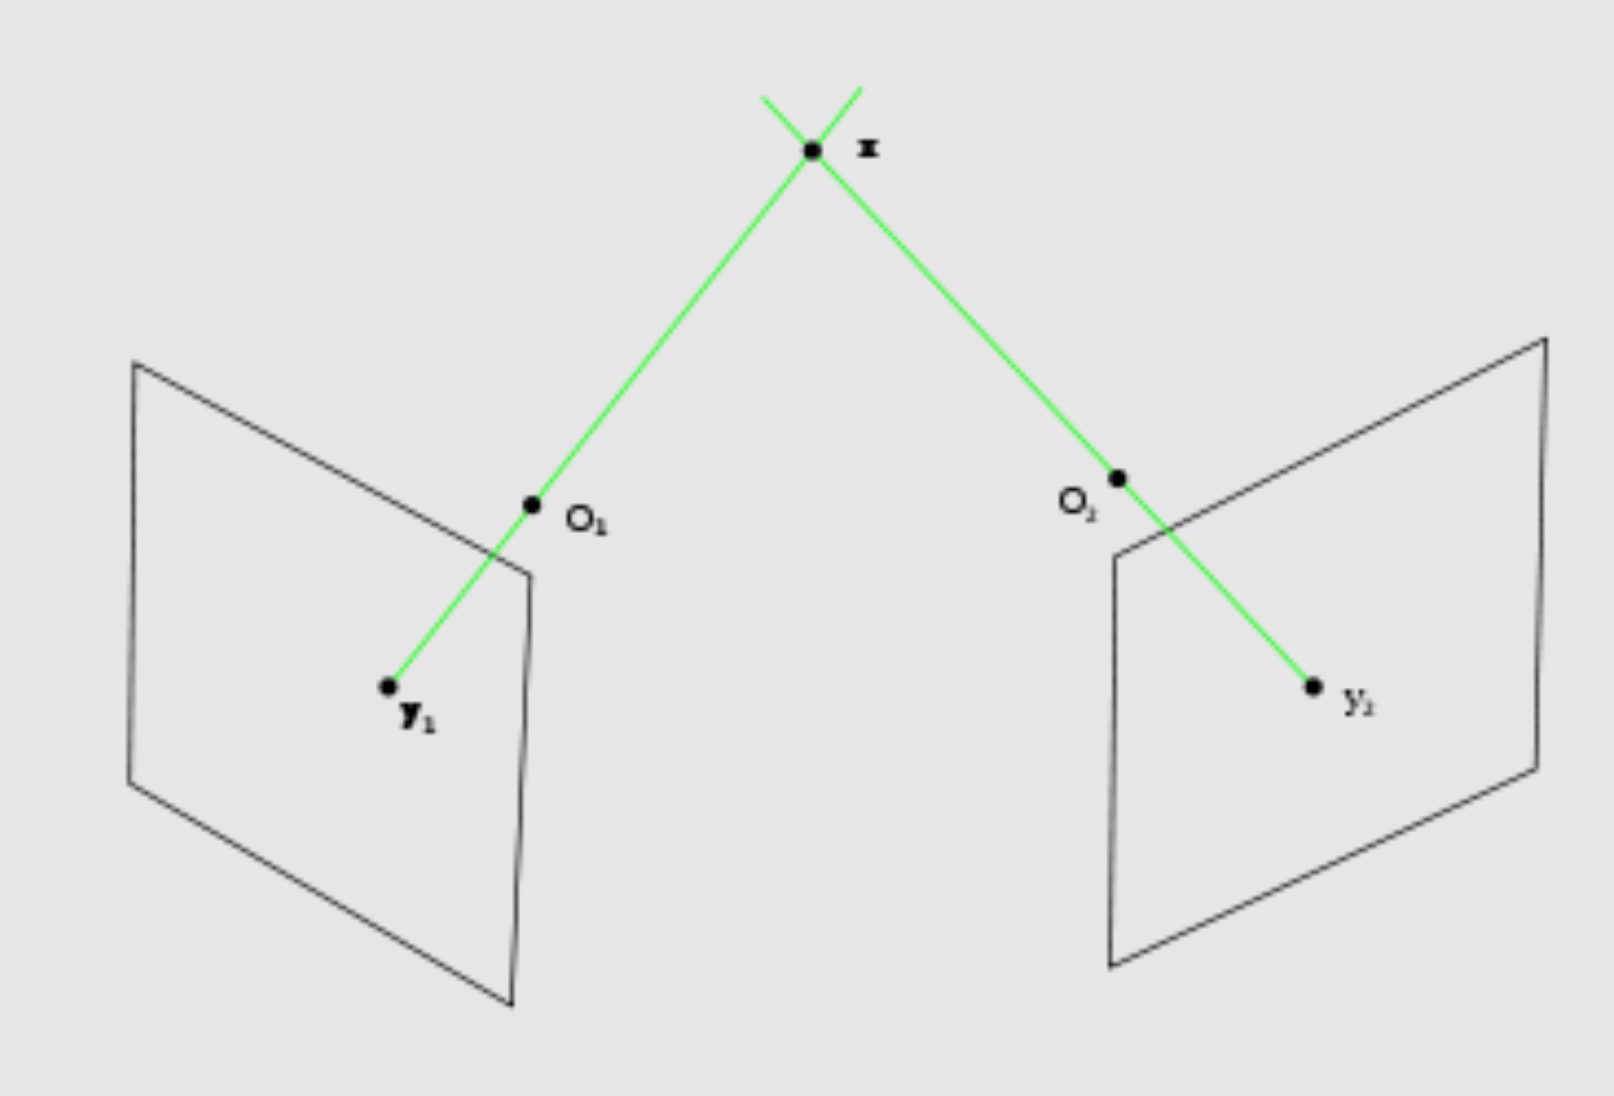
\includegraphics[height=4cm]{Res/Triangulation.png}


Der Grund warum die Pixel der „Schablone“ im Projektor zufällig angeordnet sind liegt darin, dass die unterschiedlichen lokalen Nachbarschaftsbedingungen die Pixelzuordnung zwischen dem statischen und dem dynamisch veränderten Bild erleichtern.


\subsection{Das Schattenproblem}

Aufgrund der Entfernung der verbauten RGB Kamera zur Infrarot Kamera weisen die Bilder beider Kameras einen kleinen Versatz auf.
Schatten im Tiefenbild entstehen aufgrund der Entfernung des Infrarotprojektors zur Infrarotkamera. Der Schatten im Muster macht es für den Sensor unmöglich die Tiefe festzustellen. Daher werden die Pixel in diesen Regionen auf den Wert 0 gesetzt.\\


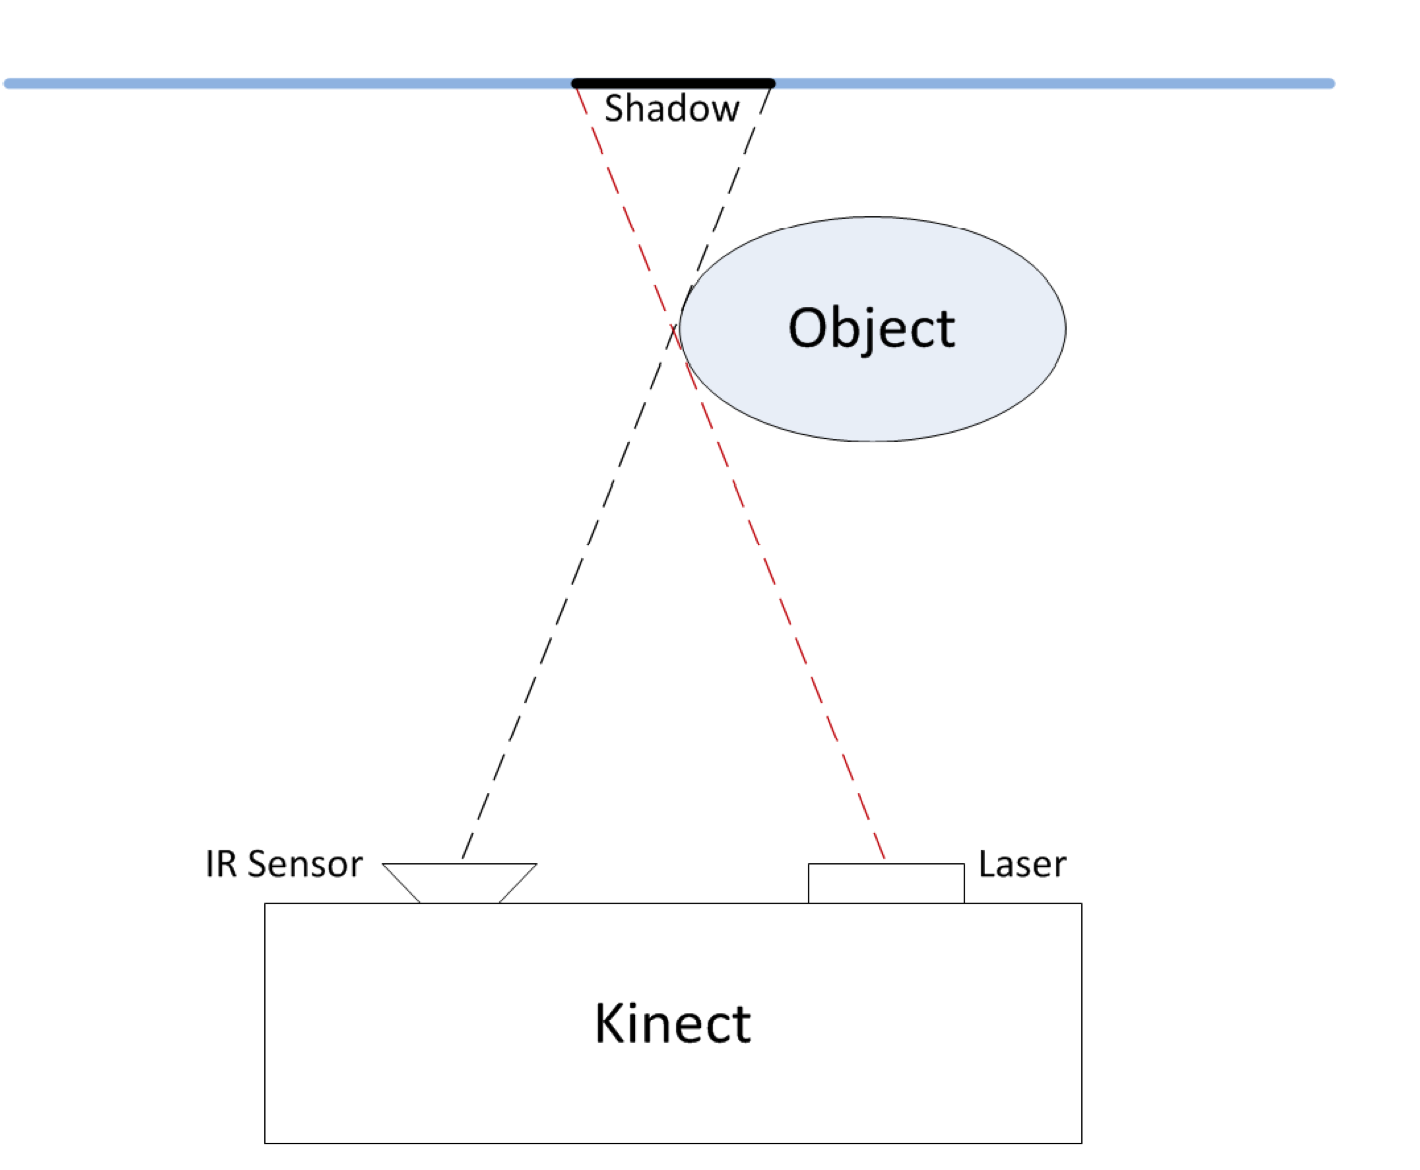
\includegraphics[height=4cm]{Res/Schatten_Strahl.png}


Das Objekt blockiert die Strahlen des Lasers. Da für die Tiefenberechnung das vom IR-Projektor emittierte Musters benötigt wird, ist es für die Kinect unmöglich die Distanz in Bereichen zu berechnen welche außerhalb der Erreichbarkeit des IR Strahlenmusters liegen. \\

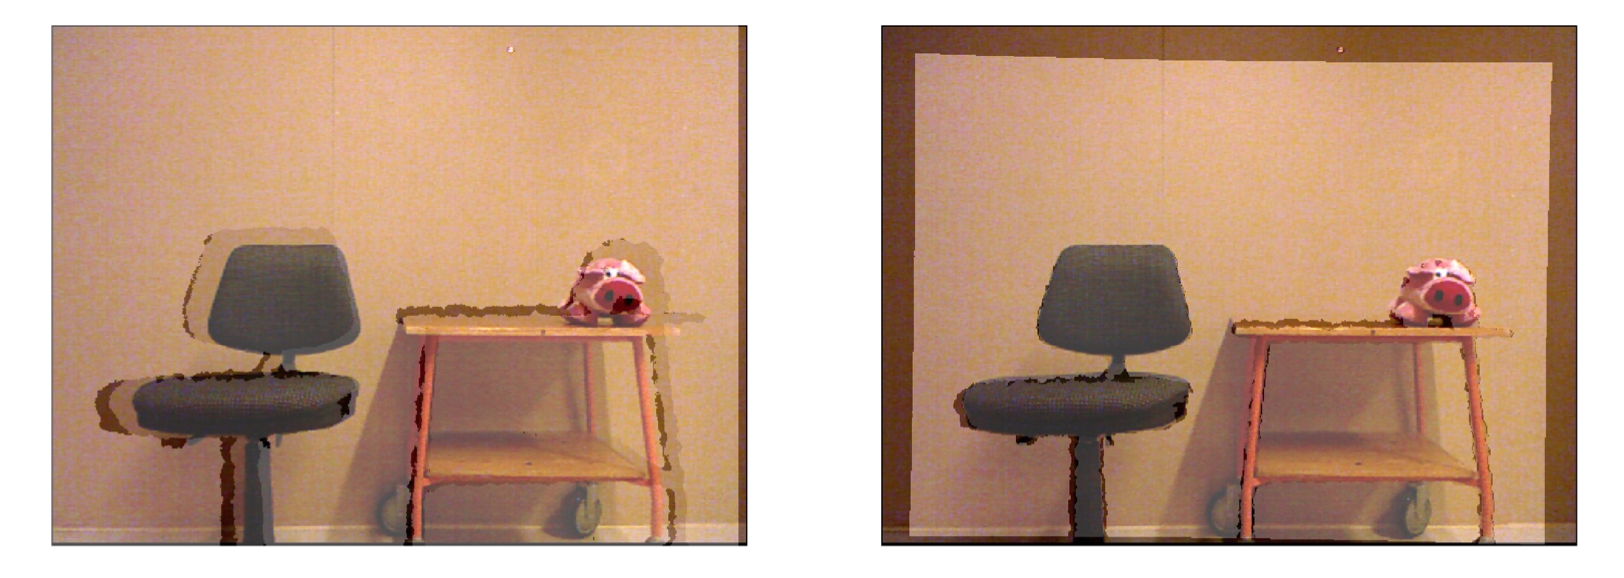
\includegraphics[height=4cm]{Res/Schatten.png}


Da der Infrarot Sensor links des Projektors positioniert ist, treten die Schatten auch linksseitig der Objekte auf. 


\section{Anforderungen}

\chapter{Die Skelettierung}
\section{Thinning}

Das Thinning bezeichnet eine Kategorie von Methoden zur Skelettierung von 2D sowie 3D Objekten. In dieser Projektarbeit ist der Fokus ausschliesslich auf die 2D Skelettierung gerichtet, da die Kinect kein vollkommenes 3D Modell eines Objektes liefert. Sie erfasst das Objekt lediglich aus einem Blickwinkel, desshalb erhält man nur ein 2,5 dimensionales Modell. Es werden nur Tiefeninformationen bezüglich Seite des Objektes, welche der Kinect zugewendet ist bereitgestellt. Die  Tiefeninformationen der Rückseite bleiben verborgen. Um ein vollständiges 3D Modell zu erhalten müssten mindestens 2 Kinects verwendet werden und die Informationen beider Geräte zusammengeführt und vereinheitlicht werden. 

Alle Thinning Algorithmen verbindet das iterative Abtragen des Musters oder der Oberfläche.

\section{Distanztransformation}
%Sandra: Theorie über Skelettierung mit der Distanztransformation
\section{Weitere Verfahren}
\section{Verwandte Arbeiten}
\subsection{Extracting Skeletons From Distance Maps}
%Sandra
\subsection{A Fast Parallel Algorithm for Thinning Digital Patterns} 


Der Algorithmus ist insgesamt in mehrere Iterationen unterteilt. Die Randpixel des Musters werden Schicht für Schicht abgetragen. Die Iterationen sind selbst wiederum in mehrere Subiterationen unterteilt. Das Abtragen der „Schichten“ wird somit in zwei unterschiedliche Phasen aufgespalten
Mit Hilfe der ersten Subiteration werden sowohl Süd- und Ostgrenzpunkte als auch Nordwest Eckpunkte entfernt. \\


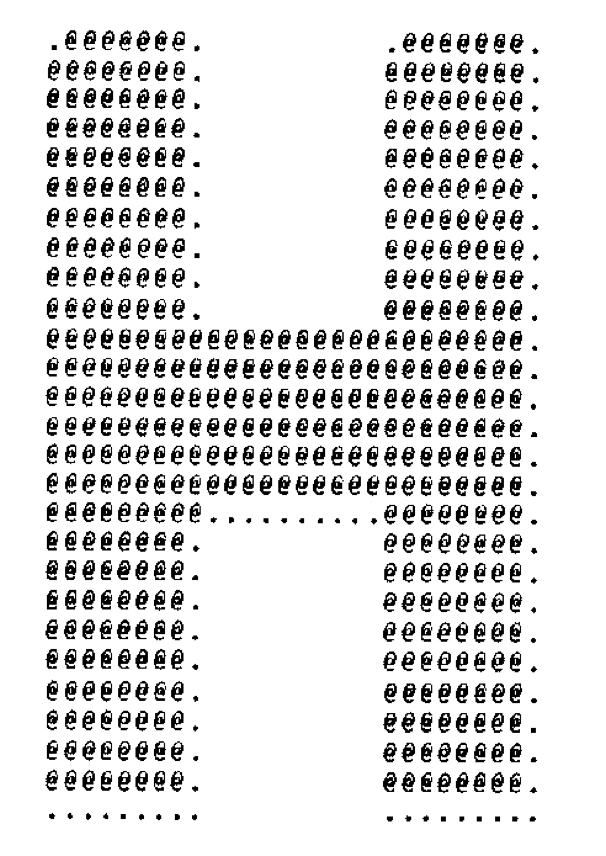
\includegraphics[width=4cm]{Res/SuedOst.png}


Das entfernen von Nord- und Westgrenzpunkten sowie von Südosteckpunkten erfolgt in der zweiten Subiteration.\\

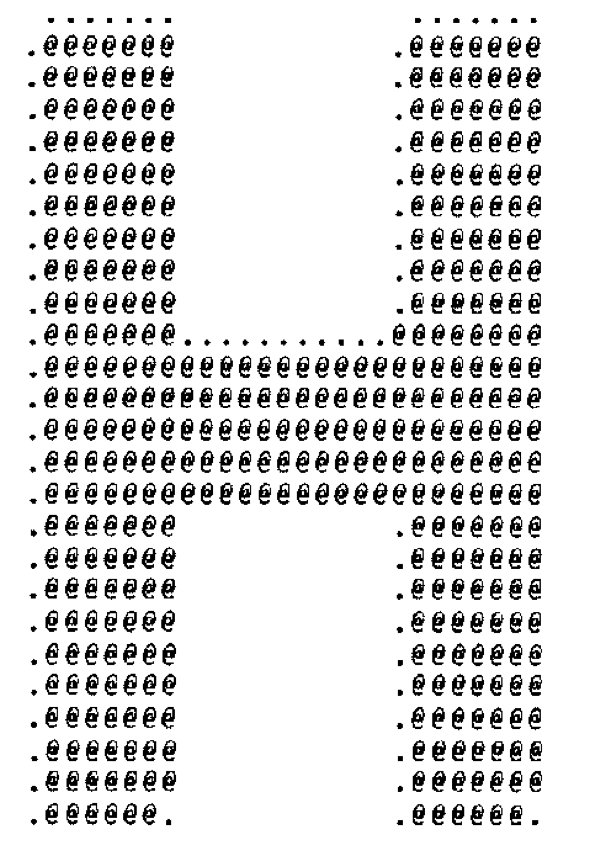
\includegraphics[width=4cm]{Res/NordWest.png}

\subsubsection{Anforderungen an den Algorithmus}

Das Rauschen, welches der Algorithmus verursacht soll so gering wie möglich gehalten werden.
Das Skelett des Ursprungsmusters soll die Endpunkt- und Pixelverbundenheit erhalten.
Endpunktverbundenheit bedeutet, dass sich zwischen zwei Endpunkten eines Skeletts keine unverbundenen Stellen befinden.
Das Skelett soll nach Durchlaufen des kompletten Algorithmus in einheitlicher Dicke von einem Pixel vorliegen.
Der Algorithmus soll möglichst schnell und effizient arbeiten um Echtzeitfähigkeit gewährleisten zu können.\\


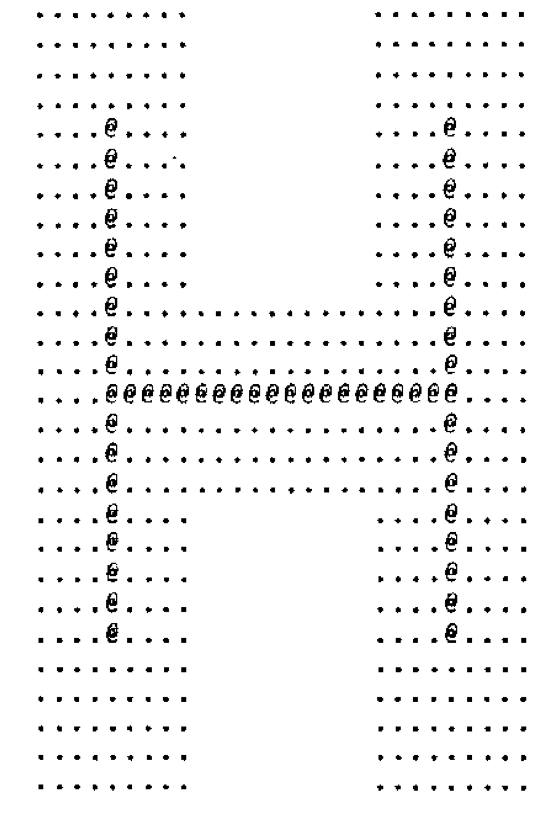
\includegraphics[width=4cm]{Res/Skelett.png}

\subsubsection{Ablauf des Algorithmus}

Es wird davon ausgegangen zu Beginn ein binär digitalisiertes Bild vorliegen zu haben.
Die Pixel werden mit Hilfe einer zweidimensionalen Matrix IT durchlaufen, deren Wert an der jeweiligen Stelle IT(i,j) entweder 0 oder 1 ist.
Mit Muster ist die Menge an Pixeln gemeint, welche den Wert eins haben.
Es werden nun in Abhängigkeit von den 8 Nachbarpixeln, Punkt für Punkt iterative Transformationen auf die Matrix angewendet.

Der neue Wert eines Pixels während der n-ten Iteration hängt von dem eigenen Wert während der (n-1)ten Iteration und den Werten der acht Nachbarn während der (n-1)ten Iteration ab. Dies ermöglicht paralleles Transformieren mehrerer Bildpunkte. 
Die Bedingungen, welche zum Ausführen der Transformation erfüllt sein müssen werden über ein 3x3 Pixel Fenster abgefragt. Der Punkt P1 über dessen Transformation entschieden wird, ist mit allen acht Nachbarn verbunden.\\

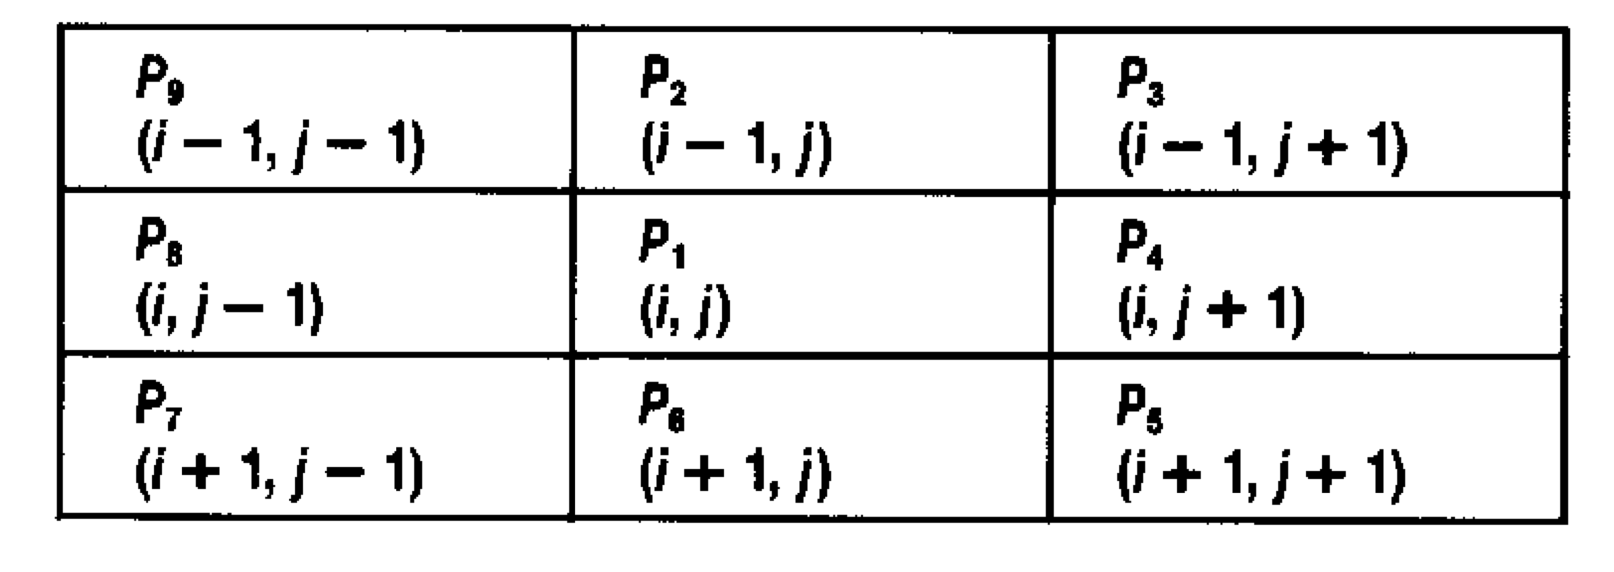
\includegraphics[width=8cm]{Res/PixelNachbarschaft.png}


Der Algorithmus entfernt alle Randpunkte des Musters, außer den Pixeln welche Bestandteil des Skeletts sind. Um die Verbundenheit des Skeletts zu gewährleisten wird ein  Iterationsschritt in zwei Subiterationen aufgeteilt.

In der ersten Subiteration wird der Punkt P1 aus dem Muster gelöscht wenn er folgende Bedingungen erfüllt:\\ \\
a)2<=B(P1)<=6     
Bà Anzahl der Nachbarn von P1 !=0
Die Anzahl der Nachbarn von P1 welche den Wert 1 haben, muss somit zwischen 2 und 6 liegen.\\ \\
b) A(P1)=1
AàAnzahl der „01“-Folgen 
Die Anzahl der 01 Folgen in der geordneten Folge P2,P3...P9 muss genau eins betragen.\\ \\
c) P2*P4*P6=0  
Mindestens ein Pixel der Pixelmenge P2, P4, P6 muss den Wert Null haben.\\ \\
d) P4*P6*P8=0
Mindestens ein Pixel der Pixelmenge P4, P6, P8 muss den Wert Null haben.
\\

Sind alle Bedingungen a, b ,c und d erfüllt so wird der Wert des Pixels auf 0 gesetzt.
Dies bedeutet dass er kein Teil des Skelett-Musters mehr ist.
Wird eine der Bedingungen nicht erfüllt, so bleibt der Pixelwert bei 1.\\

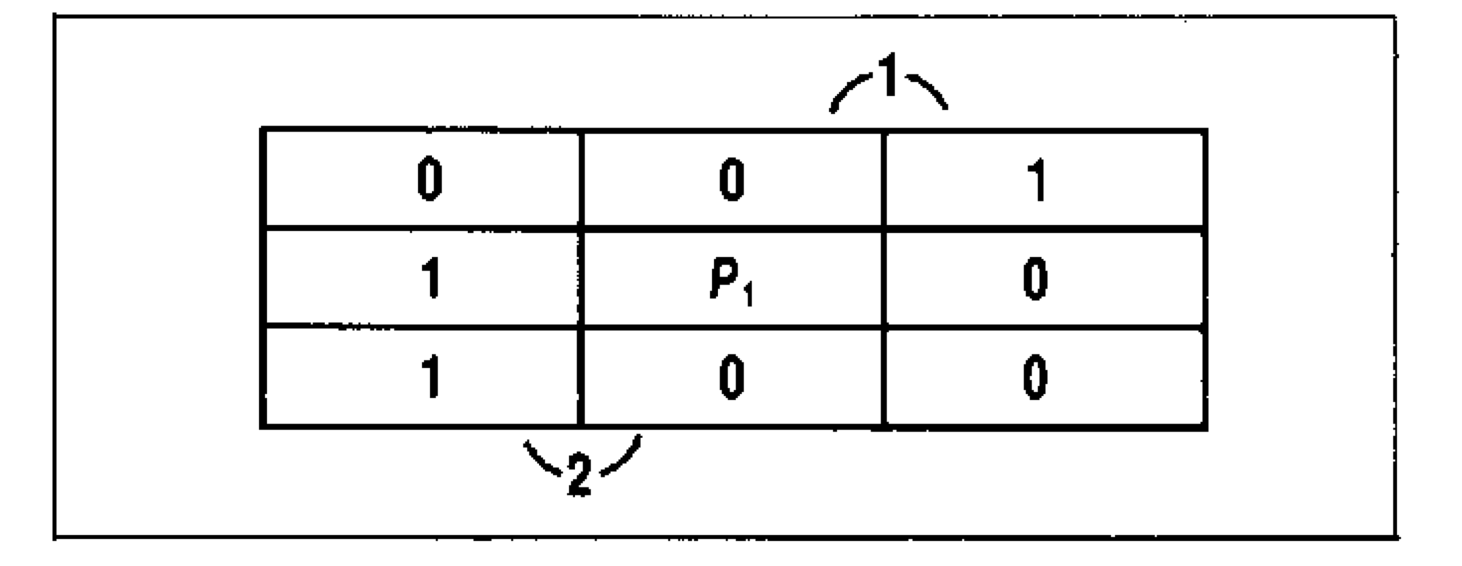
\includegraphics[width=8cm]{Res/01Folgen.png}


In der zweiten Subiteration wird P1 gelöscht falls folgende Bedingungen gelten: \\ \\
a) 2<=B(P1)<=6 \\ \\
b) A(P1)=1 \\ \\
c) P2*P4*P8=0 \\ \\
d) P2*P6*P8=0 \\ \\
In der zweiten Subiteration haben sich nur die Bedingungen c und d geändert.\\

Um die Bedingungen der ersten Subiteration zu erfüllen muss
P4=0 oder P6=0 oder (P2=0 und P8=0)  erfüllt sein.
Dies impliziert dass P1 entweder Süd- oder Ost-Grenzpunkt, oder Nordwesteckpunkt ist.
Um die Bedingungen der zweiten Subiteration zu erfüllen muss
P2=0 oder P8=0 oder (P4=0 und P6=0) sein.
Das heißt P1 ist Nord -oder West-Grenzpunkt oder Südosteckpunkt ist.

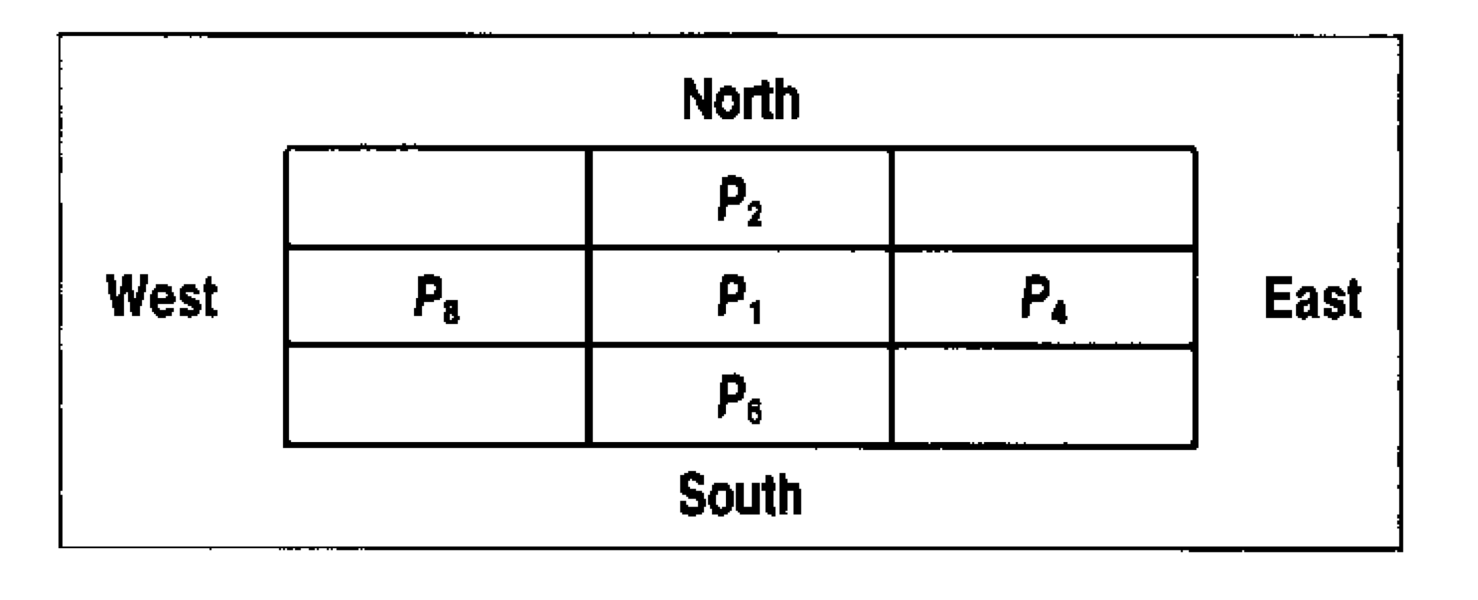
\includegraphics[width=8cm]{Res/Orientierung.png}


Während mit Bedingung a (2<=B(P1)<=6) die Endpunkte des Skeletts erhalten werden, so wird mit Bedingung b (A(P1)=1) die Auslöschung von Punkten zwischen den Endpunkten der Skelettlinie verhindert.\\

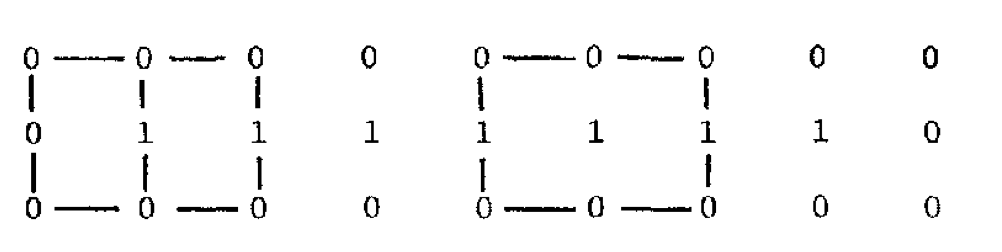
\includegraphics[width=8cm]{Res/EndpktVerbheit.png}

In der Matrix Search M befinden sich während der ersten Iteration alle Pixel die gelöscht werden dürfen, da sie den Bedingungen der ersten Iteration genügen. Ist dies nicht der Fall, so ist der Counter=0 und der Algorithmus beendet, da es anscheinend keine zu löschenden Pixel mehr gibt. Die Skelettierung ist somit beendet.
Falls der Counter ungleich null ist, werden die Pixel welche den Bedingungen genügen von der Matrix IT (Skelett-Muster) abgezogen, der Counter wird null gesetzt und es wird zur zweiten Iteration fortgeschritten. Dort findet der Ablauf mit veränderten Bedinungen c und d nochmals statt. Ist auch nach dem Durchlaufen der zweiten Subitertation der Counter ungleich null so wird der Vorgang iterativ fortgeführt.\\




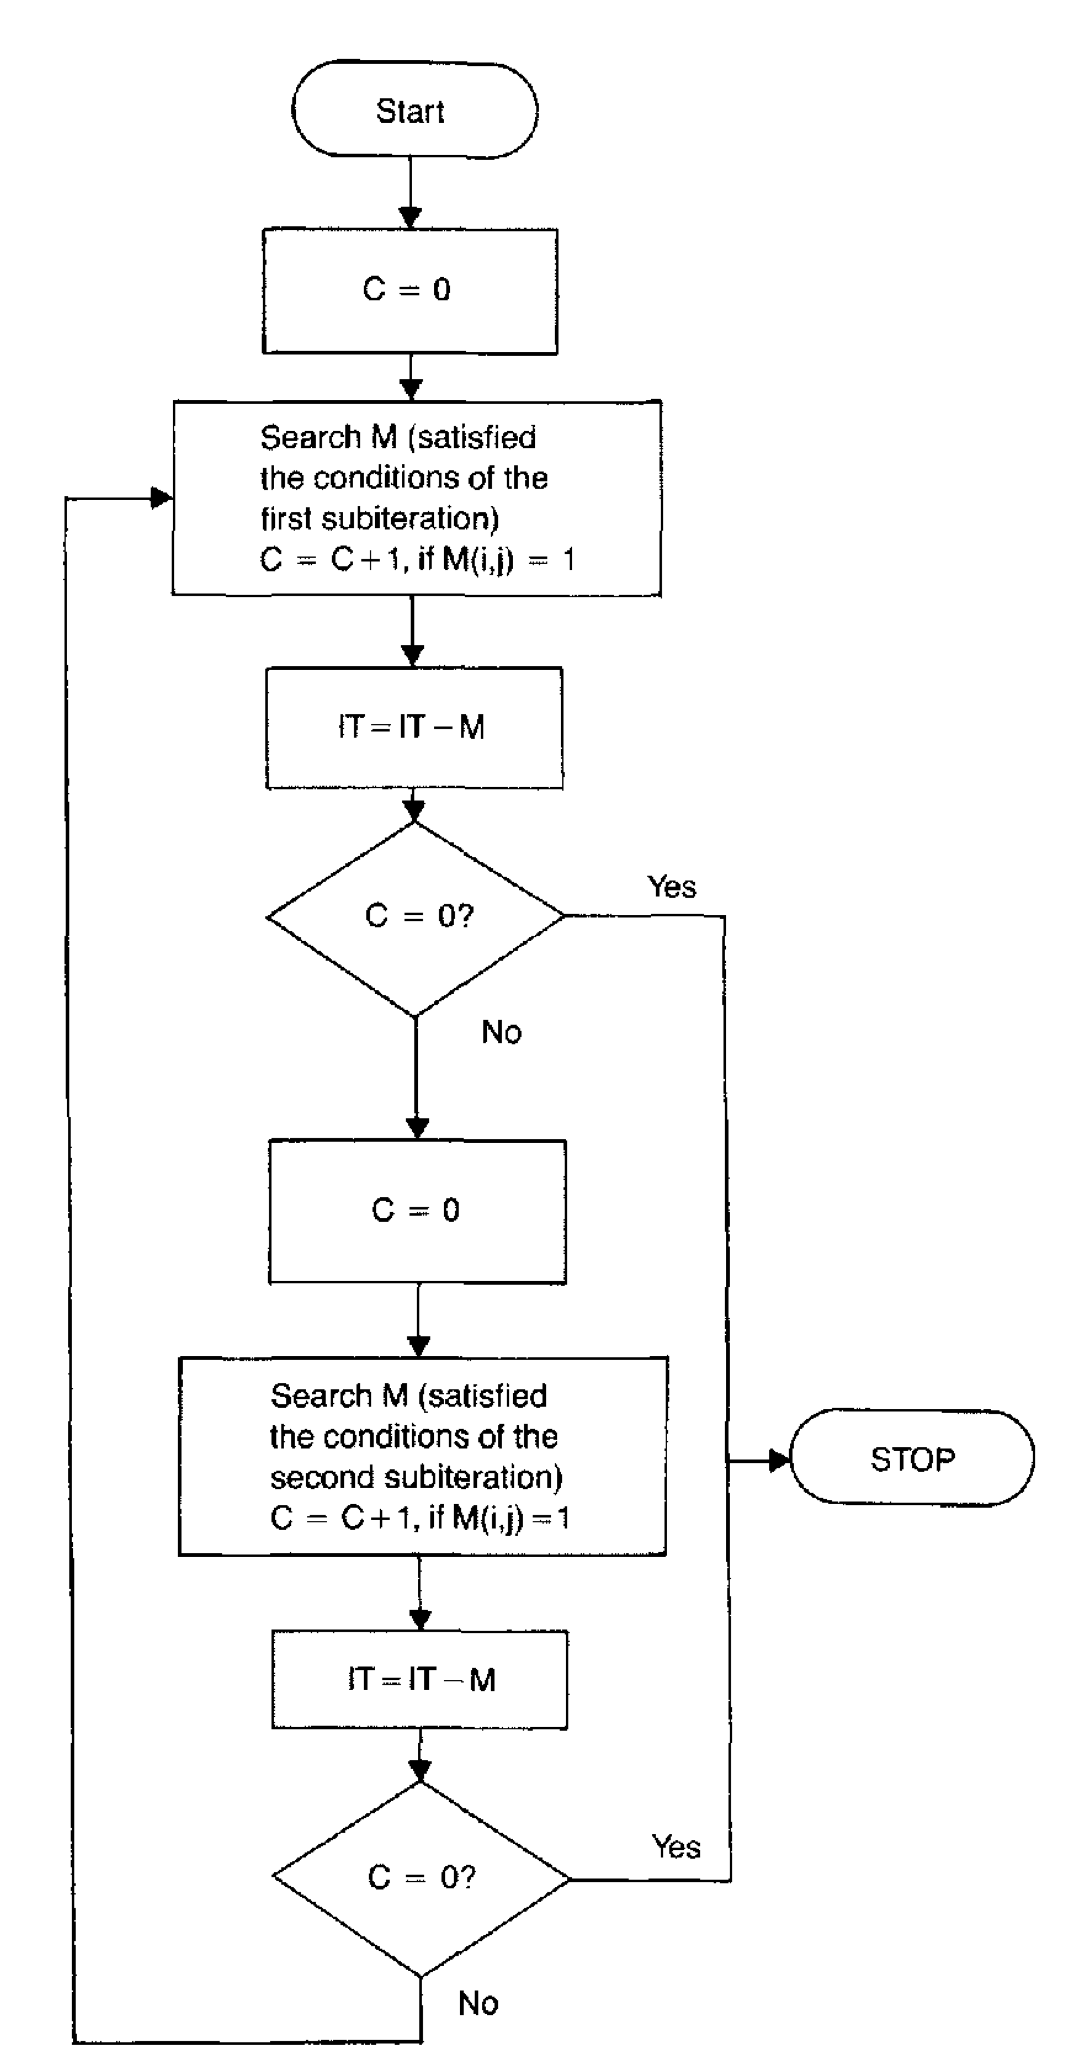
\includegraphics[width=6cm]{Res/AlgUebersicht.png}


Der Algorithmus erzielt sehr gute Ergebnisse im Bezug auf Verbundenheit, und Rauschsicherheit bei Randpunkten. Die Bedingungen welche zum Auffinden der zu löschenden Randpunkte führen sind sehr simpel. Durch den Bezug auf die n-1te Iteration zur Abfrage der Bedingungen kann der Algorithmus sehr schnell ausgeführt werden, da keine Warteabhängikeiten bestehen.



\chapter{Implementierung der Algorithmen}
\section{Wahl der Algorithmen}
\section{Die Arbeitsumgebung}
\section{Spieler-Segmentierung}
%TODO: Tiefeninformation, Verbesserung des Tiefenbilds, Nachbesserung des segmentierten Bildes -> Dilatation
%Sandra
\section{Thinning}




\section{Distanztransformation}
%Sandra
\chapter{Ergebnisse}
%Sandra
%TODO: Kriterien für den Vergleich der Algorithmen -> Eigenschaften eines Skeletts, Laufzeit
%TODO: Anwendung programmieren?
\begin{itemize}
	\item Vergleich der Algorithmen
	\item Anhand der Kriterien
	\begin{itemize}
		\item Erhaltung der Topologie
		\item Pixelkonnektivität
		\item Zentriert
		\item 1 Pixel breit
	\end{itemize}
	\item Echtzeitfähigkeit -> Messungen machen -> Vergleich
	\item Verbesserung des Skeletts (Distanztransformation) mit Breitensuche um Pixelkonnektivität zu erreichen -> Weitere Verbesserungen? -> Ohne Features sondern anhand der weißen Pixel
	\item Anwendung: Vergleich von Posen -> Features bestimmen. Vllt sowas wie "Spannweite" der Pose in x und in y Richtung (Abstand des "linkesten" zum "rechtesten" Pixel). 
\end{itemize}
\chapter{Zusammenfassung}
\chapter{Fazit und Ausblick}
\section{Fazit}
\section{Ausblick}
\chapter{TODO Anhang}
Tabelle: Wer hat was geschrieben?\\
Vollständiger Quellcode
\end{document}
